\documentclass[10pt,a4paper,oneside]{article}
\usepackage[UKenglish]{isodate}% http://ctan.org/pkg/isodate
\usepackage{amsmath}
\usepackage{url}
\usepackage{dirtree}
\usepackage{graphicx}
\usepackage[parfill]{parskip}
\usepackage{listings}
\usepackage{comment}
\usepackage{tabularx,ragged2e}
\usepackage{makecell}
\usepackage[paper=A4,pagesize]{typearea}
\usepackage{afterpage}
\setlength{\parindent}{0pt}
\graphicspath{./}
\newcolumntype{L}{>{\raggedright\arraybackslash}X}

\newenvironment{changemargin}[3]{%
\begin{list}{}{%
\setlength{\topsep}{0pt}%
\setlength{\leftmargin}{#1}%
\setlength{\rightmargin}{#2}%
\setlength{\textheight}{#3}%
\setlength{\footskip}{5cm}%
\setlength{\listparindent}{\parindent}%
\setlength{\itemindent}{\parindent}%
\setlength{\parsep}{\parskip}%
}%
\item[]}{\end{list}}

\addtolength{\oddsidemargin}{-1cm}
\addtolength{\evensidemargin}{-1cm}
\addtolength{\textwidth}{2cm}

\addtolength{\topmargin}{-1cm}
\addtolength{\textheight}{4cm}
 
\begin{document}

\title{eTarget Technical Documentation}
\author{
	Rob Dunne\\
	\texttt{rob.dunne@manchester.ac.uk}
	\and
	Anja Le Blanc\\
	\texttt{anja.leblanc@manchester.ac.uk}
	}
\maketitle

\tableofcontents
\newpage

\section{Application structure}

	The web application is an AngularJS UI interacting with a Java REST API. The data processing for parsing CSV files into the database is done using a 
	Python (version 3) script, run on a cronjob. A data flow diagram is included in Appendix \ref{appendix:diagram} along with a file tree of the web application in Appendix \ref{appendix:filetree}.
	
	\subsection{UI}
	
	The User Interface (UI) is built using AngularJS v1.6.3. Additional JavaScript libraries have been used including jQuery, and shims for IE support. These are contained in the /js directory.
	
	The UI is built as a single page application (SPA), so all HTML is contained either within the index.jsp file, or in the /includes directory. Included files are fetched with the ng-include attribute and are checked for user permission by the API first.
	
	The URLs for dev, test, and prod are:
	\begin{itemize}
		\item Dev: uomdevetarget.azurewebsites.net \\(old: decmttarget.azurewebsites.net)
		\item Test: decmtetarget.digitalecmt.com
		\item Prod: christieetarget.digitalecmt.com
	\end{itemize}
	
	\subsection{API}
	
	The REST API consists of JSP files (data.jsp, component.jsp) which act as routers to the relevant Java classes and methods. Each API endpoint has its own class, 
	and inherits generic methods for user permissions and database interactions from the parent API class. No Java frameworks are used and the files are structured 
	based on a standard Tomcat application set up / OOP.
	
		
	In addition to the JSP base API there is now also a native Java Rest API. This development was required as JSP can handle only GET and POST requests but not DELETE. 
	
	\subsection{Data API}
	
	All API calls for data are routed through api/data.jsp, with parameters passed to determine what to fetch. This endpoint should only return JSON data. 
	A user permission check is done when fetching data.
	
	\subsection{Component API}
	
	All API calls for a web component (a small piece of HTML) are done through api/component.jsp, with parameters passed to determine what to fetch. 
	This endpoint should only return HTML. A user permission check is done when fetching HTML.
	
	\subsection{Java API}
	
	Endpoint: \verb|/rest/report/{specimen_id}/{run}| \\HTTP method: DELETE 
	
	Deletes the specifid report, if the user has permission otherwise returns error code 403.
	
	Endpoint:  \verb|/rest/pdf/{name.pdf}| \\HTTP method: GET
	
	Accesses the specified PDF, if the user has permission otherwise returns error code 403. 
	
	\subsection{Data processing}
	\label{sec:data_processing}
	
	The data processing VM handles all incoming files and data from the clinical partners, and copies PDFs to a secure storage area, 
	and CSV data to the database. This is a separate Linux VM from where the web application is hosted. 
	
	A Python script (targetdata.py) is called once a minute via cron that fetches files and data and redistributes them. 
	The Python script can be found in the ./targetdata directory in the home folder of the VM.
	
	Cron job rg\_Target\_Dev, TargetData VM: /var/spool/cron/crontabs (crontab -e as the user)\\
	Shell script rg\_Target\_Dev, TargetData VM: /home/commander/target\_data/\allowbreak run.sh
	
	\subsection{Database}
	
	Data is often split across multiple tables in the database (database schema in Appendix~\ref{appendix:db_schema}) - 
	the initial schema was defined based on a previous project - so check for foreign keys when tracking data. Common data requests, 
	such as a list of patient data, are aggregated in views for more simplified SQL queries.

\section{Infrastructure}
	This project runs on Azure cloud services provided by CRUK. Please contact Paul Fitzpatrick for access\footnote{Paul Fitzpatrick, \url{mailto:Paul.Fitzpatrick@digitalecmt.org}}.
	
	\subsection{App Service}
	
	The App Service is a Tomcat server that hosts the web application.
	
	\subsection{Data processing VM}
	
	The VM is a Linux server that processes files that are added to the file storage. 
	PDF files are copied to configured secure storage area in a configured directory (Table: \ref{tab:table1}). CSV files are processed for patient 
	data which is added to the database. No data is stored on the VM.
	
	\subsection{File storage}
	
	The file storage is accessed by the data uploaders. Files uploaded are copied by the VM and then deleted. 
	Access is by Azure Storage Explorer\footnote{Azure Storage Explorer, \url{https://azure.microsoft.com/en-gb/features/storage-explorer/}} 
	using the access key found in the Azure control panel.
	
	A second storage area is used as the premanent location for uploaded PDF files.
	
	\subsection{Database}
	
	Standard SQL server and SQL database. The patient ID reference is encrypted using Triple DES. 
	The encryption key is stored in the \verb|eTargetVault| (Key Vault) in the \verb|DECMT_DEV_eTarget| Resource group.
	
	You will need to add your IP address to the firewall whitelist in Azure to access the database.

\section{First set up}
\subsection{Virtual Machine}
This section assumes a Azure Administrator has created a barebone Linux VM. The only task for the VM is to run a python script in regular
intervals (every minute). The set up consists of installing all required Python libraries, setting up the configuration file, and creating a 
cron job for the regular runs.

\subsubsection{Setup SSH access to VM}
SSH access to the VM is required firstly to set it up, but also to keep the VM updated. Steps:
\begin{enumerate}
  \item Log into Azure
  \item Find the VM in 'Resource Groups' or 'Virtual Machines'
  \item In the section for 'Support and Troubleshooting' select 'Reset Password'
  \item Choose 'Reset SSH public key'
  \item Choose a user name and copy your public key into 'SSH public key' field.
\end{enumerate}
For ease of use I have set up an alias in .bash\_aliases with the IP address of the VM found on the Azure portal.

To gain root access on the VM do \verb|sudo bash|.

It is advisable to run an update of the operating system before continuing to install new software.

The service VMs are set up, so that you need to open the firewall for certain time before you can ssh into them.
In the Security Centre of the Azure Portal you find the 'Advanced Cloud Defense' with an item 'Just in time VM access'. 
Find your VM in there, tick the checkbox and click the button 'Request access'; select port 22 and click 'Open ports'.
A short time late you'll gain access.

\subsubsection{Create a service account for running python}
\label{sec:useraccout}

Idealy you want an service account (\verb|useradd -r commander|) for the user running the python script in a cron job. But this was not done on any of our environments and
for consistency reasons we go for a normal user account which can't be used for login.
\begin{verbatim}
useradd commander
usermod -L commander
\end{verbatim}
This means the user still got a home directory \verb|/home/comander| and an associated shell (\verb|/bin/bash|).

\subsubsection{Install Python libraries}

Install python libraries as the user who should run them, i.e. commander. That means only this user can execute those libraries.
\begin{verbatim}
pip3 install 'azure-storage-blob==1.1.0'
pip3 install 'azure-storage-file==1.1.0'
pip3 install pymssql
#pip install crypto
pip3 install pycryptodome
pip3 install 'openpyxl==2.6.4'
pip3 install pycel
pip3 install ftpretty
pip3 install zlib
pip3 install jsonschema

yum install zlib-devel
\end{verbatim}

As an admin install

\verb|apt-get install python3-crypto|

\subsubsection{Configure python script}

The python script requires a \verb|.config| file for its configuration. This file is not part of the git repository as it contains sensitive information.
The basic structure is:
\verb|key; value|.

For the list of keys see Table~\ref{tab:table1}.

\begin{table}[ht!]
  \setlength\extrarowheight{2pt}
  \begin{center}
    \caption{Table of required keys for the configuration}
    \label{tab:table1}
    \begin{tabularx}{\textwidth}{|l|L|L|} % <-- Alignments: 1st column left, 2nd middle and 3rd right, with vertical lines in between
      \hline
      \textbf{Key} & \textbf{Description} & \textbf{Where to find}\\
      \hline
      remotehostname & DNS name of database server & Azure portal; SQL database; Overview; Server name\\
      remoteusername & User name to access the DB & Azure portal; DECMT\_DEV\_eTarget resourcegroup; eTargetVault; Secrets; find the right db \\
      remotepassword & password to remoteusername & Azure portal; DECMT\_DEV\_eTarget resourcegroup; eTargetVault; Secrets; find the right db \\
      remotedbname & Name of the database & Azure portal; SQL database; SQL databases\\
      fileuser & Username for storage where users upload data files to (i.e. the data directory) & Azure portal; Storage account; Settings; Access keys; storage account name\\
      filekey & Access key for that storage account & Azure portal; Storage account; Settings; Access keys; key1 or key2 key\\
	  patientkey & Is used to encrypt and decrypt the Christie patient number & Azure portal; DECMT\_DEV\_eTarget resource group; eTargetVault; Secrets; Encryption Key\\
      storageurl & Connection string to the storage account & Azure portal; Storage Account; Settings; Access keys; use connection string\\
      containername & Name directory in blob usually 'reports' & will be created
      if not existent\\
      logblob & Name of the blob container for log files & create with the file explorer or in the Azure portal\\
      \hline
    \end{tabularx}
  \end{center}
\end{table}

\subsubsection{Setup cron job for python script}

The python script should run as the user created in section \ref{sec:useraccout}.
\begin{verbatim}
sudo bash
su commander
crontab -e
\end{verbatim}
Add the line (adapt to the correct location):

\verb|*/1 * * * * bash /home/commander/target-data/run.sh /dev/null 2>&1|

and save. This runs the run.sh script every minute. The script itself makes sure it is not running more than once, i.e. if the ingestion takes longer than a minute.

\subsection{Database}
There is currently no SQL script for setting up an empty eTarget database. Therefore you currently have to copy an existing eTarget database 
(from the Dev or Test environment) to the new Database Service and clean out the existing data. 

\subsection{Storage}
Create a file share \verb|data| on Azure portal or via a Storage Explorer.

Create a blob share \verb|log| on Azure portal or via a Storage Explorer.

\subsection{Application}

Please read the sections \ref{sec:build}, \ref{sec:deploy}.

For a new environment add a server section as described in \ref{sec:build}.

In \verb|pom.xml| create a new profile section. See table~\ref{tab:table2} for explainations of the \verb|<properties>|.

\begin{table}[ht!]
  \setlength\extrarowheight{2pt}
  \begin{center}
    \caption{Table of required properties in pom.xml \textless profile\textgreater ~section}
    \label{tab:table2}
    \begin{tabularx}{\textwidth}{|l|L|L|} % <-- Alignments: 1st column left, 2nd middle and 3rd right, with vertical lines in between
      \hline
      \textbf{property} & \textbf{Description} & \textbf{Where to find}\\
      \hline
	  serverid & given id in .m2/settings.xml & see that file\\
	  postfix & name of the war file is \verb|etarget|+postfix\verb|.war| & set here\\
	  azureFtpUrl & in case the deploy to the azure environment happens via sftp (wagon plug-in), this is the URL used & Azure portal; App service; Overview; FTP hostname + /sites/wwwroot\\
	  webapp.include.path & where to find the include directory on the web server; note: this changes between Windows and Linux hosts & Azure portal; App service; Advanced Tools/SSH; than look for location\\
	  databaseURL & JDBC url for connecting with the DB & \makecell[l]{\verb|jdbc:jtds:sqlserver://| \\ + Server name + \verb|/| \\ + db name;  Server name \\ and db name can be \\ found in Azure portal; \\ SQL database; Overview}\\
	  dbuser & User name which the web-app should use & Azure portal; DECMT\_DEV\_eTarget resourcegroup; eTargetVault; Secrets; find the right db\\
	  dbpassword & Password for dbuser & Azure portal; DECMT\_DEV\_eTarget resourcegroup; eTargetVault; Secrets; find the right db\\
	  storageURL & Location of PDF files & Azure portal; Storage account; Access key; Connection string\\
	  \makecell[l]{RESOURCE \\ GROUP\_NAME} & Info about your Azure subscription; used for azure maven deploy & az webapp list\\
	  WEBAPP\_NAME & Name for this webapp in Azure; used for azure maven deploy & az webapp list\\
	  REGION & Region in which the webapp is deployed; used for for azure maven deploy & az webapp list\\
	  web.path & Path to the web app on the server; if on root use \textbackslash & your choice\\
      \hline
    \end{tabularx}
  \end{center}
\end{table}

\subsubsection{Configurations}

Configurations are split into three config files:
\begin{enumerate}
  \item application.properties -- contains application relevant settings
  	\begin{enumerate}
  	  \item \verb|edit.timeout| setting of the edit timeout in minutes; after that number of minutes an edit-locked patient will be released. 
  	  \item \verb|application.version| sets ver version string for the browser tab name; value taken from \verb|pom.xml|.
  	  \item \verb|application.title| Name of the application as shown on the browser tab
  	  \item \verb|application.imageURL| Footer image URLs, comma separated, either relative URLs into the eTarget application or absolute URLs to other web resources
  	  \item \verb|application.imageAlt| Alternative text for imates, displayed for screen readers or when images fail to laod
  	  \item \verb|application.support| Email address on site to request help
  	  \item \verb|data.blood| whether blood data is available
  	  \item \verb|data.tumour| whether tumour data is available
  	  \item \verb|page.additional_reports| display additional reports tab
  	  \item \verb|page.ihc| display IHC tab
  	  \item \verb|page.fmblood| display FM Bloods tab
  	  \item |verb|page.fmtumour| display FM Tumour tab
  	  \item \verb|page.tumourngs| display Tumour NGS tab
  	  \item \verb|page.ctdnangs| display CtDNA NGS tab
  	  \item \verb|page.ctdnaexploratory| display CtDNA Exploratory tab
  	  \item \verb|page.pdxcdx| display PDX CDX tab
  	  \item \verb|page.name| comma separated list of providers as found in the eTarget database table \verb|CONCEPT_DATASOURCES| column \verb|panel_name|
  	  \item \verb|page.name.[name1]| name which should be displayed for this provider
  	  \item \verb|page.name.[name1].blood| whether blood tab should be displayed
  	  \item \verb|page.name.[name1].tumour| whether tumour tab should be displayed
  	  \item \verb|page.name.[name1].code| two letter code which will be used for this provider in reports 
	\end{enumerate}
  \item config.properties -- contains connection settings
    \begin{enumerate}
      \item \verb|serverid| Maven setting in \verb|.m2/settings.xml| which contains the login data (username + password) the server
      \item \verb|azureFtpUrl| The URL to use in case deployment is done using FTP (caused problems and generally moved to azure maven deploy)
      \item \verb|toWarFile| The location for which the war file is to be build; needs to match where to deploy in Apache
  	  \item \verb|databaseURL| URL to the database; value taken from \verb|pom.xml|. 
  	  \item \verb|dbuser| user name for the database; taken from \verb|pom.xml|.
  	  \item \verb|dbpassword| password for dbuser; taken from \verb|pom.xml|.
  	  \item \verb|storageURL| URL to Azure blob storage (location of the PDFs); taken from \verb|pom.xml|.
  	  \item \verb|storageContainerName| Name of the blob 'folder' for reports (PDFs)
  	  \item \verb|trialContainerName| Name of the blob 'folder' for trial HTML documents (generated from the trail finder)
  	  \item \verb|webapp.include.path| location of the include folder on the web server; taken from \verb|pom.xml|.
  	  \item \verb|RESOURCEGROUP_NAME| Name of the Azure resource group for Maven Azure deploy; taken from Azure portal
  	  \item \verb|WEBAPP_NAME| Name of the Azure web application; taken from Azure portal
  	  \item \verb|REGION| Name of the deploy region; note: do not take from the Azure portal, required is the short name \verb|az| client provides, the one without spaces and catital letters.
  	  \item \verb|PRICING| Pricing of the web application; taken from the Azure portal
  	  \item \verb|SUBSCRIPTION_ID| Id of the subscription; taken from the Azure portal
  	  \item \verb|web.path| location of where it should be deployed
	\end{enumerate}
  \item logging.properties -- standard logging properties file; set logging levels
\end{enumerate}

\subsection{Active Directory}

Authentication is done using Microsoft's Active Directory service. This needs to be configured on the Azure portal. This part is best done by the administrator of Azure.

Enable Authentication: Azure Portal: go to the correct App Service; Authentication/Authorization; switch on 'App Service Authentication'.\\ 
Use Azure Active Directory: 'Action to take when request is not authenticated': 'Log in with Azure Active Directory'.\\
'Authentication Providers': configure Azure Active Directory. Management Mode:
Advanced. \\

Client ID: Copy from Azure portal; Azure Active Directory; App registration; Application ID\\
Issuer URL: \verb|https://sts.windows.net/|+ Azure portal; Azure Active Directory;  Properties; Directory ID\\
 

\section{Code repository}
	A copy of the web application code is hosted on the UoM Research IT Github repository\footnote{eTarget, \url{https://github.com/UoMResearchIT/TARGET}}. A separate repository exists for the data processing code, also on the UoM Research IT Github\footnote{Data processing, \url{https://github.com/UoMResearchIT/target-data}}.
	
	Robert Haines\footnote{Robert Haines, \url{mailto:robert.haines@manchester.ac.uk}} at Research IT can provide access to these repositories.
	
\section{Build}
\label{sec:build}
	\begin{comment}
	The Java API needs to be compiled before being deployed to the server if any changes are made. 
	In the WEB-INF/classes directory you will find a build.sh file. Update the relevant path in this file, 
	then run to compile / build the API. JSP, CSS, JS, and HTML file changes can be sent straight to the 
	server. 
	\end{comment}

	Building is done using maven. There are currently three profiles defined: dev, test, prod. 
	Before building check the content of those environments. The project settings are expected in a directory 
	'profiles' with a sub-directory named as the profile name.
	
	\begin{lstlisting}  % Start your code-block
	
 <servers>
   <server>
     <id>etarget_dev_app</id>
     <username>USERNAME_AZURE</username>
     <password>PASSWORD_AZURE</password>
   </server>
   <server>
     <id>etarget_test_app</id>
     <username>USERNAME_AZURE</username>
     <password>PASSWORD_AZURE</password>
   </server>
   <server>
     <id>etarget_prod_app</id>
     <username>USERNAME_AZURE</username>
     <password>PASSWORD_AZURE</password>
   </server>
 </servers>
	\end{lstlisting}
	
	Information about server location, usernames, and passwords can be found in the Azure Portal 
	$(App Service \rightarrow Get Publish Profile.)$
	
	\verb|id| is a identifier you choose and will refer to in \verb|pom.xml|. 
	
	\verb|username| is a combination of {\it msdeploySite}\textbackslash{\it userName} 
	
	\verb|password| is \textit{userPWD}
	
	Command to build i.e. a dev web application:
	\begin{lstlisting}
	mvn clean package -Denv=dev
	\end{lstlisting}

	Assuming everything runs OK this produces etarget\_dev.war file in the target directory. Ready to deploy!	
	
	\subsection{Building with Java Overlays}
	
	Java Overlays is a way to overwrite part of your application with different files. This is of advantage when building for several clients with 
	slightly diverging needs, i.e. diverging naming conventions for elements in the UI, different logos and such. Currently the configuration files 
	are kept in an overlay structure so not to compromise access to DB details.
	
	Creating an Overlay requires a separate project. Files which should be overwritten by this overlay need to be located at the same
	directory location as in the original project. So if you want to overwrite the file \verb|\profiles\prod\config.properties| you need to create
	that file in that location in the new project.
	
	In the \verb|pom.xml| you need to add etarget as and dependency of the new project:
	\begin{lstlisting}
<dependencies>
	<dependency>
		<groupId>org.digitalecmt</groupId>
		<artifactId>etarget</artifactId>
		<version>2.0-SNAPSHOT</version>
		<classifier>classes</classifier>
	</dependency>
	<dependency>
		<groupId>org.digitalecmt</groupId>
		<artifactId>etarget</artifactId>
		<version>2.0-SNAPSHOT</version>
		<type>war</type>
	</dependency>
</dependencies>
	\end{lstlisting}
	Note: there are two dependencies, one for the Java classes, and one for the war file. Make sure that you build against the right version of etarget!
	
	Otherwise you should define your profiles in the same way as in the base project and you need to define your build plugins and resources as 
	needed.
	
	Building has to be done in two steps:
	\begin{lstlisting}
	mvn install -Denv=[env] 
	\end{lstlisting}
	on the TARGET repository
	\begin{lstlisting}
	mvn package azure-webapp:deploy -Denv=[env]
	\end{lstlisting}
	on the new Overlay repository.
	
	The first command installs the built base eTarget package into the local Maven repository, so that the second build process can find and use
	it.

\section{Deployment}
\label{sec:deploy}

	\begin{comment}
	Deployment to the dev environment is via 'push to deploy' continuous integration from the Github repository. Pushing a new update to the repo will trigger the App Service to pull and deploy the latest code.
	
	You will need to visit the dev App Service section in Azure, and login to the repo with your Github login details under the 'Deployment options' section.
	
	Deployment to test and production are via SFTP to prevent accidental deployment of development code. You may wish to change this for easier deployment.
	\end{comment}

	Deployment to all environments can be done via maven, i.e. for the dev environment:
	
	\begin{lstlisting}
	mvn install -Denv=dev
	\end{lstlisting}
	
	This uses the \verb|wagon-maven-plugin| to upload the war file to the configured server using ftp. Running this goal for the first time on an empty
	App Service will cause an error as it tries to delete directories which do not yet exist. One way around this is to disable the install goal remove 
	part of the plugin for the first run. Alternatively just create the directories so that the plug-in has something to delete.
	
	On a Linux based App Service the deploy by ftp does not work. In this cases there is a second way to install a war file. Please check for spelling 
	issues carefully as this will create Azure services if it can't find them!
	
	\begin{lstlisting}
	mvn package azure-webapp:deploy -Denv=dev
	\end{lstlisting}
	
	Uses the \verb|azure-webapp-maven-plugin| to deploy the web app. (After the packageing goal a specific deploy goal is called.) There are different configurations required for a Windows based Application server 
	than for a Linux one!
	
	Alternatively you could use any other deploy method provided by Azure. The aim is to get the etarget\_\$env.war file into the webapps folder of the correct server. Tomcat takes over the deployment of the war file on the server.
	
	Deployment of code to the processing server VM is via SSH / SCP / git. 

\section{Access}

	Please contact Paul Fitzpatrick for a copy of the spreadsheet with login details for test and production.
	
	Paul will also need to create accounts for you in Azure to access the dev VM (SSH) and Azure AD (to login to the frontend).
	
	SFTP login details can be found in the Azure control panel for the relevant App Service, or in the application code config files - please email me to request these as they are not in the repo.

\section{Known issues}
	
	The following are a list of known issues in that may not be documented in JIRA. 
	
	\begin{itemize}
		\item Distro mismatch for the data processing VMs. The previous sysadmin set up the wrong distro for test and production. Dev is running Ubuntu, whereas test and prod are running RHEL. Please be aware of this when installing / updating packages, deploying code, or debugging.
	\end{itemize}

\section{Appendix}
\appendix
\section{Application data flow diagram}
\label{appendix:diagram}
\bigskip
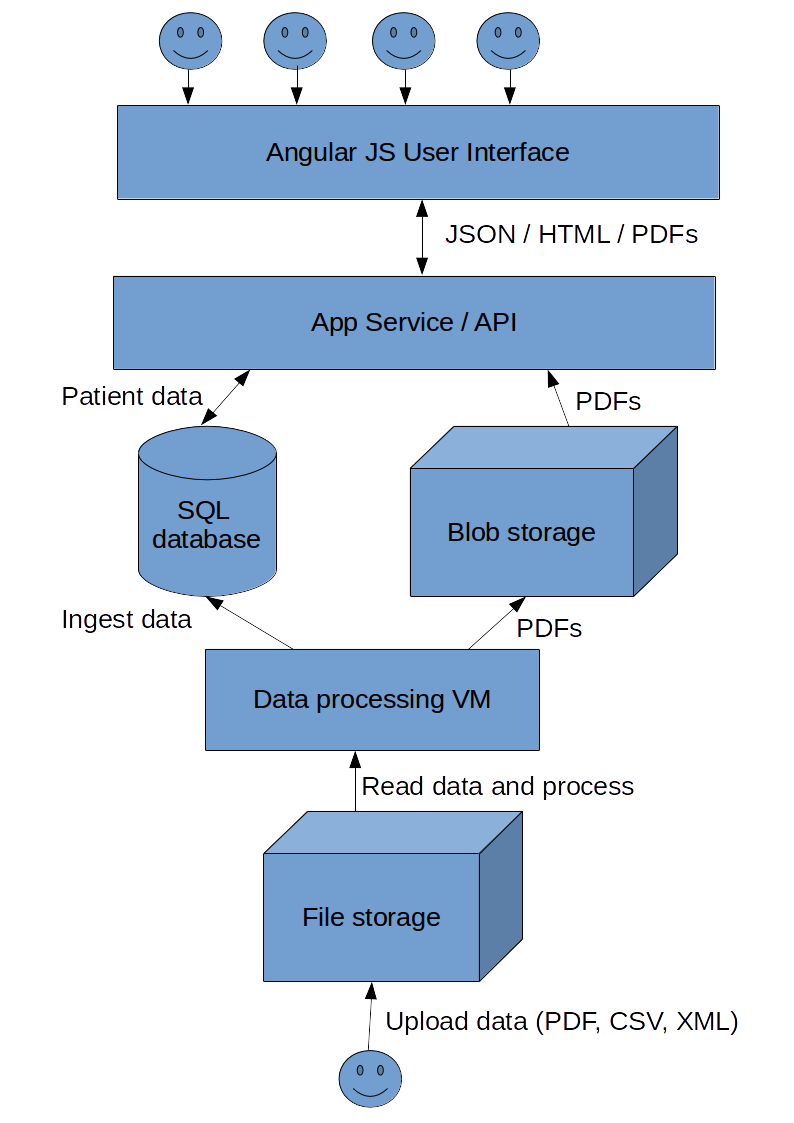
\includegraphics[width=\textwidth, height=0.9\textheight, keepaspectratio]{FlowDiagram} 
\afterpage{% Insert after the current page
\KOMAoptions{paper=A3,pagesize}
\recalctypearea
\begin{changemargin}{-3cm}{-5cm}{36cm}
\section{DB schema eTarget version 1.0}
\label{appendix:db_schema}
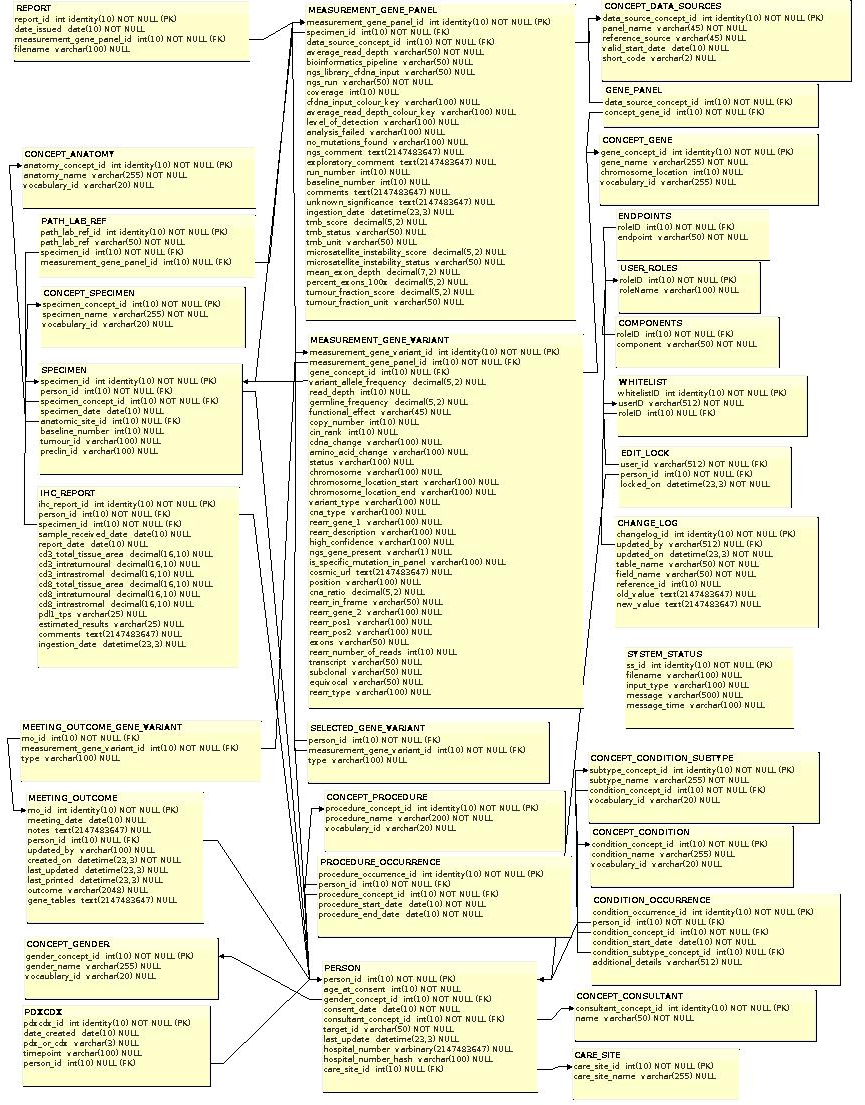
\includegraphics[height=\textheight,width=1.3\textwidth,keepaspectratio]{OpenSourceDB} 
\end{changemargin}
\clearpage
\KOMAoptions{paper=A4,pagesize}
\recalctypearea
}
\newpage
\section{Web application structure}
\label{appendix:filetree}
% Include a tree diagram of application
	\dirtree{%
	  .1 /webapps.
	  .2 /ROOT.
	  .3 index.jsp.
	  .3 logout.jsp.
	  .3 /css.
	  .4 pikaday.css.
	  .4 style.css.
	  .4 mobile.css.
	  .3 /images.
	  .4 example.png.
	  .3 /js.
	  .4 angular.min.js.
	  .4 moment.js.
	  .4 notice.js.
	  .4 pikaday.js.
	  .4 inactivity.js.
	  .4 app.js.
	  .3 /includes.
	  .4 ctdnangscheckbox.html.
	  .4 admin.html.
	  .4 adminlink.html.
	  .4 reportextraction.html.
	  .4 tumourcheckbox.html.
	  .4 patienttable.html.
	  .4 meetingoutcome.html.
	  .4 ctdnaexpcheckbox.html.
	  .4 \ldots.
	  .3 /WEB-INF.
	  .4 /classes.
	  .5 /org.
	  .6 /digitalecmt.
	  .7 /etarget.
	  .8 compiled\_class\_files.
	  .5 config.properties.
	  .5 application.properties.
	  .5 logging.properties.
	  .4 /lib.
	  .5 gson-2.8.0.jar.
	  .5 jtds-1.3.1.jar.
	  .5 jollyday-0.5.1.jar.
	  .5 \ldots .
	  .3 /api.
	  .4 component.jsp.
	  .4 data.jsp.
	}

\end{document}